\documentclass[11pt]{article}
\usepackage{amsmath, amssymb}
\usepackage{hyperref}
\usepackage{graphicx}
\usepackage[margin=1in]{geometry}
\usepackage{verbatim}
\usepackage{wrapfig}

% Define \problemname and \illustration if not using Kattis template
\newcommand{\problemname}[1]{\section*{#1}}
\newcommand{\illustration}[3]{%
    \begin{figure}[h]
        \centering
        \includegraphics[width=#1\textwidth]{#2}
        \caption{#3}
    \end{figure}
}

\begin{document}

\section*{1. Topics Chosen}

We started with the idea of candy trading with someone whose preferences were hidden, which we
decided was more interesting/challenging than a standard optimization
problem. Solving our problem uses two strategies. The first is learning Bob's
values from his replies, which uses \textbf{Complete Search} over the possible values.
The second is using that knowledge to trade as little as possible, which is
\textbf{Dynamic Programming} for the ``cheapest'' trade. There is also a third topic,
\textbf{Simulation}. Contestants must track their inventory, their Final Bowl, and the
outcome of every trade. We chose this combination because a contestant who
uses only one of the techniques gets a worse result, and so our problem
rewards using them together.

A \textbf{Greedy strategy} that always pays with the candy you value least is
tempting, but wastes the information you receive in his replies. We expect it
to fail, which makes it a useful wrong solution to include.

\section*{2. Research Summary}

The algorithm is \textbf{Interactive} because not all of the input is given at the
beginning. Instead, a handful comes at the beginning, and future output
depends on future input, which can't allow batch computing. Bob's replies
follow a fixed protocol (ACCEPT/ADD at most once/DECLINE/WALK), so the
solution is a per-listing state machine, not a single computation. This also
makes the problem an \textbf{Online Decision} problem, in which the algorithm changes
its methods in real time to incoming information.

Dynamic programming can be implemented as the \textbf{Dual Knapsack}: minimize the
total cost of selected items subject to reaching a value of at least a
target. In our problem the two value systems separate, each candy piece costs
its satisfaction $a$ to us, but its value is Bob's hidden $b_t$. Since every
$b_t$ is unknown, we set the target to the worst case over our surviving
candidate vectors $\sum(b_t \cdot c_t) > T$, so the DP returns the cheapest
offer that is guaranteed to be accepted. Reconstructing the actual bundle
from the DP table (rather than reading off a number) yields the OFFER line.

During the interaction loop, \textbf{Knuth's Mastermind} algorithm can be combined
with the knapsack to make the most revealing guess. Mastermind works very
similarly to Wordle; the goal is to guess a 4 color code with 6 color options
($6^4 = 1296$ options) in at most 10 moves, and Knuth's algorithm does it in
at most 5. First, a set of all codes is initialized, then the most revealing
guess is made, a response with correct-position-correct-colors and
wrong-position-correct-colors, then every code that doesn't match the
response gets removed, then start again with the next most revealing guess.
We could do the same in our problem, where we initialize a set of all
satisfaction values Bob could have, assume the worst-case threshold for our
knapsack, then among the offers we can afford, make the most revealing one
(found through a \textbf{Complete Search}): The offer whose ACCEPT/ADD
reply comes closest to splitting our candidate set in half. After the response,
prune every satisfaction vector inconsistent with it, and repeat.
Determining the guess uses a Complete Search over the set of all satisfaction values.

What we do have foresight on, however, is the listings. We have the option to SKIP any
listing, which begs the question: ``Can $S$ be reached without taking this
deal?'' which in itself is another \textbf{Dual Knapsack problem}, where we need to minimize
the number of offers we take to guarantee a satisfaction $\geq$ to some
goal.

\section*{3. Problem Type}

The selected problem type is \textbf{Hybrid}, specifically a mix of \textbf{Construction and
Interactive}. Our team decided to make a Construction problem because we found
that it gave us more creative freedom for possible solutions. To solve this
challenge, one could use a combination of an input-tracking loop, a greedy
algorithm, and dynamic programming. We chose to make the problem Interactive
in order to add more complexity to the challenge. Instead of knowing the
satisfaction of the other candy trader, the problem-solver needs to deduce
their satisfaction from trades.

\section*{4. Problem Statement}

\problemname{Trick-or-Trade}

\begin{wrapfigure}{r}{0.4\textwidth}
    \centering
    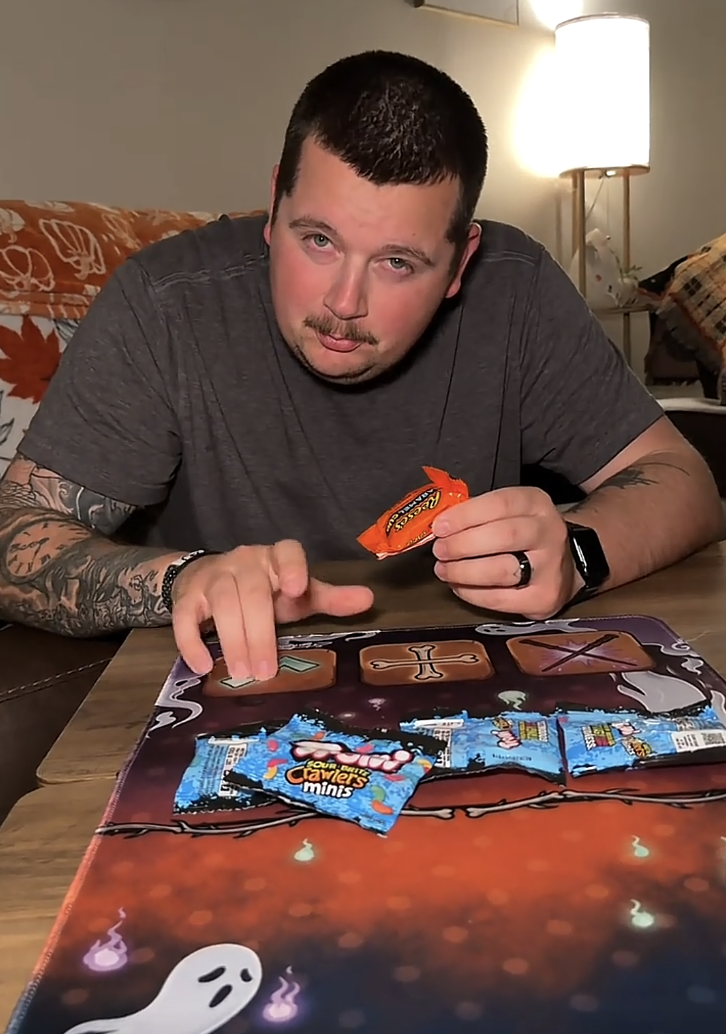
\includegraphics[width=\linewidth]{image1.png}
    \caption{Bob during the trading night}
\end{wrapfigure}

Your parents run Sweet Tooth Capital, a trading firm, and they're raising you
and your brother Bob to take over the family business one day. The training
program is simple: every Halloween, the two of you trade candy with each other
like real traders.

There's a catch. Your parents like Bob more, so they gave him control of the
trading system. Bob decides which listings get posted and in what order, and
only he knows how much he actually values each candy. If he thinks you're
lowballing, he'll tell you to add more, but only once, because Bob has very
little patience. Anything you hand over is gone for good. Anything you receive
goes into your Final Bowl, where it counts at midnight but can never be traded
again.

There are five types of candy: Starburst, Skittles, Twizzlers, Reese's Pieces
and Nerds. Each piece of type $t$ is worth $a_t$ satisfaction to you and $b_t$
satisfaction to Bob. You know your candy preferences, but Bob keeps his $b_t$
secret. All of these values are fixed before the night begins and do not
change throughout the night.

Bob has posted $N$ listings, in a fixed order. A listing is a type and a
count, meaning Bob will hand over that many pieces of that type. You know all
the listings in advance. Work through them one at a time, paying with your own
candy, and finish the night with a total satisfaction of at least $S$.

\subsection*{Input}

The first line of the input contains a single integer $S$
($1 \le S \le 10\,000$), your satisfaction goal.

Each of the next five lines contains a type name, the number of pieces $o_t$
you own ($0 \le o_t \le 100$), and your satisfaction $a_t$ per piece
($1 \le a_t \le 10$). The types appear in the order Starburst, Skittles,
Twizzlers, ReesesPieces, Nerds.

The next line contains the integer $N$ ($1 \le N \le 100$). Each of the next
$N$ lines contains a type name and an integer $c$ ($1 \le c \le 50$): this
listing is $c$ pieces of that type.

Bob's values satisfy $1 \le b_t \le 10$ for every type $t$ and are not part of
the input.

\subsection*{Interaction}

For each listing, in order, print one line:
\begin{itemize}
    \item \texttt{SKIP} to pass on the listing.
    \item \texttt{OFFER $t_1$ $c_1$ $t_2$ $c_2$ \ldots} to put $c_j$ pieces of
        type $t_j$ on the table. Each type may appear at most once, and you
        can only use candy you still own that is not in your Final Bowl.
\end{itemize}

Bob's gain is the total $b$-value of the candy you have offered minus the
total $b$-value of the candy in the listing. He replies:
\begin{itemize}
    \item \texttt{ACCEPT} if his gain is strictly positive. The candy you
        offered goes to Bob, and the listed candy goes into your Final Bowl.
    \item \texttt{ADD} otherwise, at most once per listing. Bob is asking for
        more, and you must answer with one of the following:
        \begin{itemize}
            \item \texttt{OFFER $t_1$ $c_1$ $t_2$ $c_2$ \ldots} again, with
                additional pieces that are added to your earlier offer. Bob
                then replies \texttt{ACCEPT} if his gain is now strictly
                positive, or \texttt{DECLINE} otherwise.
            \item \texttt{WALK} to withdraw from this listing. Nothing is
                traded and all the candy you offered returns to you. Bob
                replies \texttt{DECLINE}.
        \end{itemize}
    \item \texttt{DECLINE} if his gain is still not positive after your second
        \texttt{OFFER}, or after \texttt{WALK}. Nothing is traded, and your
        offered candy returns to you.
\end{itemize}

After the last listing, your program must exit. If your total satisfaction,
Final Bowl included, is at least $S$, your submission is Accepted. An invalid
line, or a total below $S$, gives Wrong Answer.

Remember to flush standard out after every line.

\begin{table}[h]
\centering
\begin{tabular}{l|l}
\textbf{Your output} & \textbf{Bob's reply} \\
\hline
\texttt{OFFER Skittles 3} & \texttt{ADD} \\
\texttt{OFFER Skittles 1 Twizzlers 2} & \texttt{ACCEPT} \\
\texttt{OFFER Nerds 1} & \texttt{ACCEPT} \\
\end{tabular}
\end{table}

For this sample, the input is

\begin{verbatim}
10
Starburst 10 4
Skittles 10 4
Twizzlers 10 2
ReesesPieces 10 5
Nerds 10 1
2
Nerds 2
Starburst 2
\end{verbatim}

Suppose Bob values each piece as $b_{\text{Starburst}} = 1$,
$b_{\text{Skittles}} = 2$, $b_{\text{Twizzlers}} = 3$,
$b_{\text{ReesesPieces}} = 4$ and $b_{\text{Nerds}} = 5$. On the first listing
(2 Nerds, worth $10$ to Bob), your offer of 3 Skittles is only worth $6$ to
him, so he asks for more. The added 1 Skittle and 2 Twizzlers bring the total
offer to 4 Skittles and 2 Twizzlers, worth $14$ to Bob, so his gain is
$14 - 10 = 4 > 0$ and he accepts. You paid $4 \cdot 4 + 2 \cdot 2 = 20$
satisfaction, but gained 2 Nerds in your Final Bowl. On the second listing
(2 Starburst), offering a single Nerd is already worth more to Bob
($5 > 2$) than the listing, so he accepts immediately. Your Final Bowl now
holds 2 Nerds and 2 Starburst, worth $2 \cdot 1 + 2 \cdot 4 = 10$
satisfaction, and the candy left in your possession is still worth $139$,
for a total of $149 \ge S$, so the submission is Accepted.

\section*{5. Candidate Solutions}

\subsection*{(a) The solutions that should be accepted by your problem}

For a solution to be accepted, the program must exit after the last listing
and must run without errors. If your total satisfaction is more than or equal
to $S$, the code will be accepted.

\subsection*{(b) The solutions that should fail your problem}

If your total satisfaction is below $S$, the program does not exit after the
last listing or the code has an error of any type, the solution is not
correct. Additionally, if the program takes longer than 3 seconds to run, it
will exceed the allowed time limit.

\subsection*{Asymptotic Complexity Analysis}

The solution needs to sort the 5 candy types by satisfaction level, and
sorting an array of 5 types could take $O(5 \log 5)$. Finding the cheapest
candy to offer to Bob initially would take $O(5)$. If Bob wants more candy
than offered, finding the next cheapest candy would take $O(5)$. This would
repeat for every listing $N$. The number of listings multiplied by the time
taken per operation would be: $N \cdot (O(5 \log 5) + O(5)) = O(N \cdot
5\log 5) \approx 12$ operations per loop. Because the number of candy types
is fixed, this runs in linear time $O(N)$. The space complexity is $O(T)$ for
the same reason, as the program only needs to store variables based on the 5
candy types.

\end{document}
